\documentclass[a4paper]{article}

\usepackage[czech]{babel} %https://github.com/michal-h21/biblatex-iso690
\usepackage[
   backend=biber      % if we want unicode 
  ,style=iso-numeric % or iso-numeric for numeric citation method          
  ,babel=other        % to support multiple languages in bibliography
  ,sortlocale=cs_CZ   % locale of main language, it is for sorting
  ,bibencoding=UTF8   % this is necessary only if bibliography file is in different encoding than main document
]{biblatex}

\usepackage[utf8]{inputenc}
\usepackage{fancyhdr}
\usepackage{amsmath}
\usepackage{amssymb}
\usepackage[left=2cm,right=2cm,top=2.5cm,bottom=2.5cm]{geometry}
\usepackage{graphicx}
\usepackage{pdfpages}
\usepackage{url}

\usepackage{siunitx}
\sisetup{locale = DE, separate-uncertainty = true} %    kdybych chtel +/-

\usepackage{float}
\newfloat{graph}{htbp}{grp}
\floatname{graph}{Graf}
\newfloat{tabulka}{htbp}{tbl}
\floatname{tabulka}{Tabulka}

\renewcommand{\thefootnote}{\roman{footnote}}

\pagestyle{fancy}
\lhead{Praktikum IV - (A5) Spektrometrie záření alfa}
\rhead{Vladislav Wohlrath}
\author{Vladislav Wohlrath}

\bibliography{source}

\newcommand{\Am}{$^{241}$Am}
\newcommand{\Puosm}{$^{238}$Pu}
\newcommand{\Pudev}{$^{239}$Pu}
\begin{document}

\begin{titlepage}
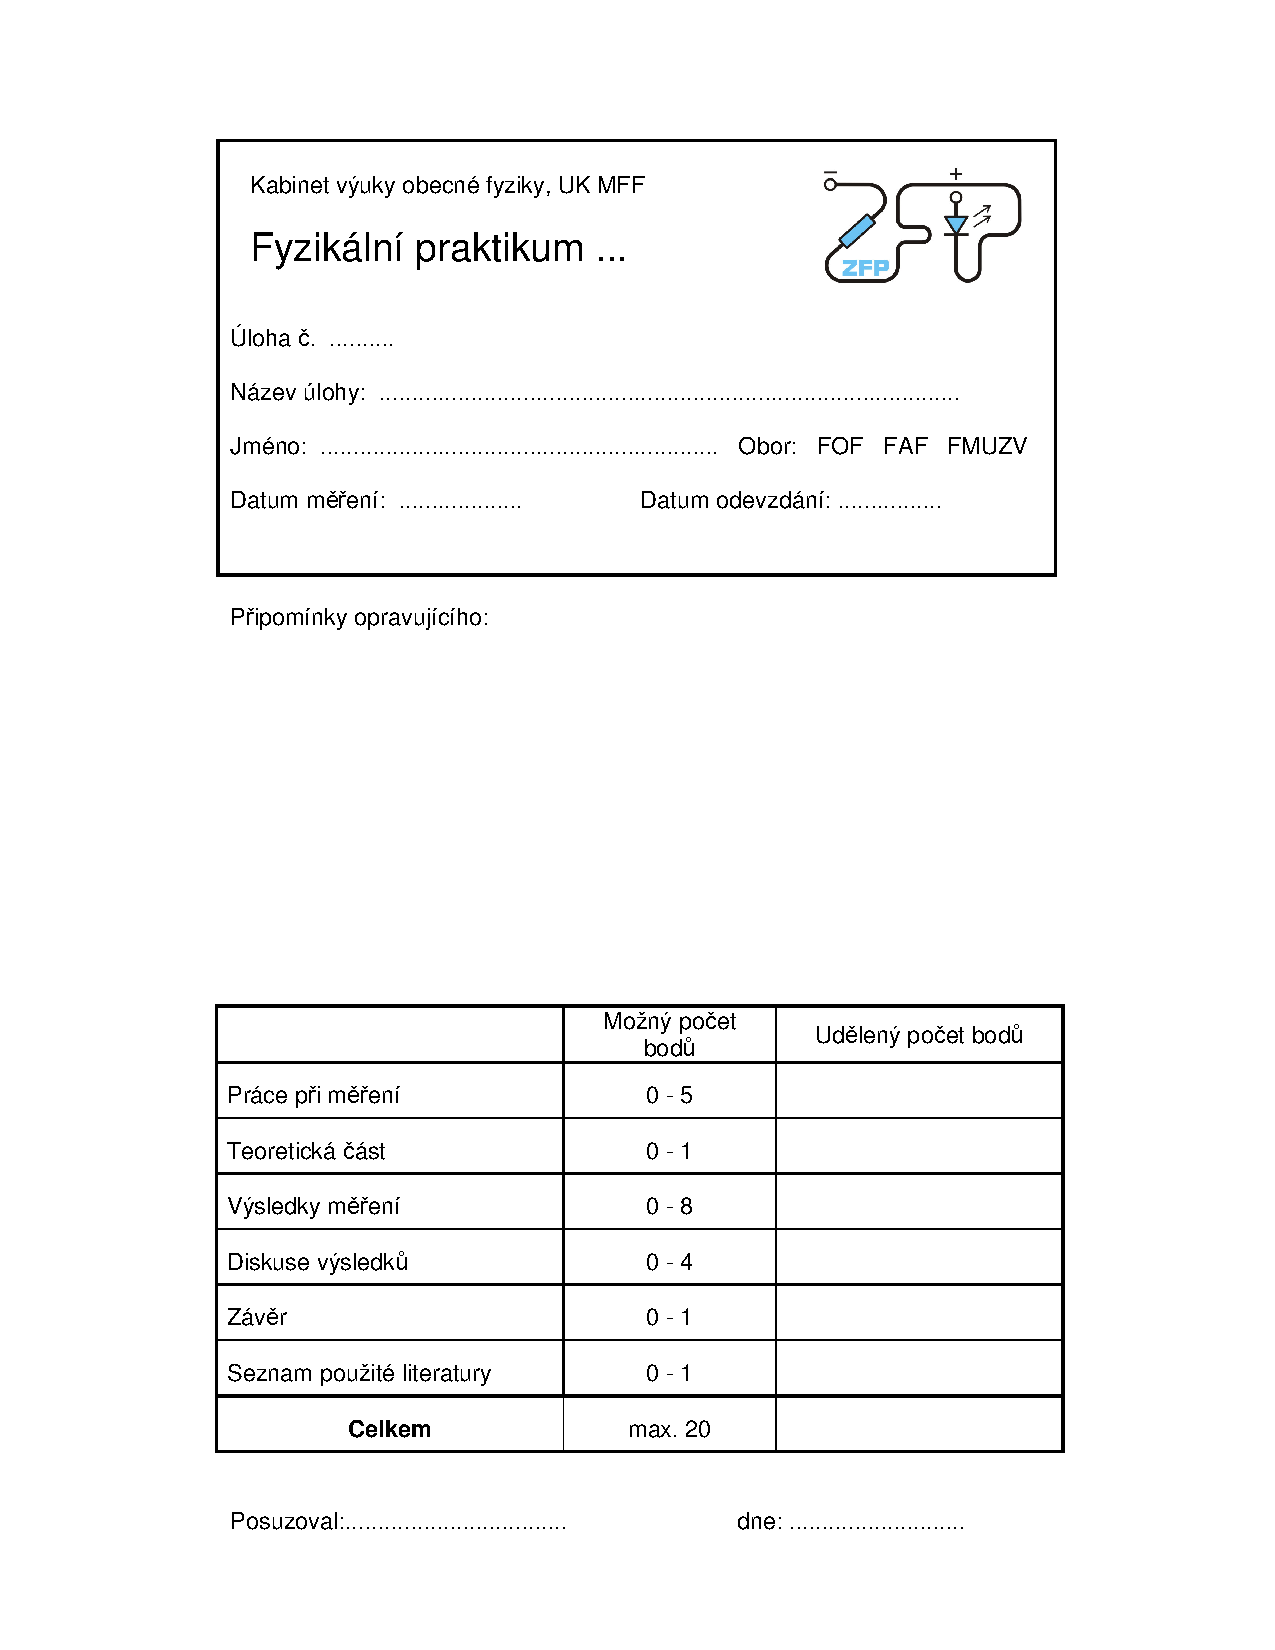
\includepdf[pages={1}]{./graficos/titlelist.pdf}
\end{titlepage}

\section*{Pracovní úkoly}
\begin{enumerate}
\item Proveďte energetickou kalibraci $\alpha$-spektrometru a určete jeho rozlišení.
\item Určete absolutní aktivitu kalibračního radioizotopu \Am.
\item Změřte závislost ionizačních ztrát $\alpha$-částic na tlaku vzduchu $\Delta T=\Delta T(P)$.
\item Určete specifické ionizační ztráty $\alpha$-částic ve vzduchu při normálním tlaku $-\frac{dT}{dx} = f(T)$. Srovnejte tuto závislost se závislostí získanou pomocí empirické formule pro dolet $\alpha$-částic ve vzduchu za normálních podmínek.
\item Určete energie $\alpha$-částic vyletujících ze vzorku obsahujícím izotop \Pudev~a příměs izotopu \Puosm~a porovnejte je s tabelovanými hodnotami. Stanovte relativní zastoupení izotopu \Puosm~ve vzorku s přesností lepší než \SI{10}{\percent}, jsou-li $T_{1/2}(^{238}\text{Pu}) = \SI{87.71}{yr}$ a $T_{1/2}(^{239}\text{Pu}) = \SI{24.13e3}{yr}$.
\end{enumerate}

%Teoretická část
\section*{Teoretická část}
Absolutní aktivita vzorku $A$ je celkový počet částic, který ze vzorku vyletí za jednotku času.
Pokud naměříme ve spektrometru aktivitu $a$, pak platí
\begin{equation}\label{aktivita}
A=a \frac{4\pi}{\Omega} \approx a \frac{r^24\pi}{S} \,,
\end{equation}
kde $\Omega$ je pokrytý prostorový úhel, $r$ je vzdálenost terčíku od vzorku a $S$ je povrch terčíku. V přiblížení $r^2 \gg S$ platí $\Omega \approx S/r^2$.


Předpokládáme, že hustota vzduchu je přímo úměrná tlaku. Potom ionizační ztráty při tlaku $P$ na vzdálenosti $r$ jsou stejné jako ionizační ztráty při atmosférickém tlaku $P_0$ a na vzdálenosti
\begin{equation}
x=r\frac{P}{P_0} \,.
\end{equation}
Specifické ionizační ztráty definujeme \cite{skripta}
\begin{equation} \label{f}
f(T):=-\frac{dT}{dx}=-\frac{P_0}{r}\frac{dT}{dP} \,.
\end{equation}
Derivaci $dT/dP$ budeme počítat numericky jako rozdíl dvou vedlejších bodů
\begin{equation} \label{dTdP}
\frac{dT}{dP}=\frac{T_{i+1}-T_i}{P_{i+1}-P_{i}} \,.
\end{equation}
Zdroj \cite{skripta} udává (po derivaci doletu částic $R$) teoretickou závislost
\begin{equation} \label{teoreticka}
f(T)=\frac{2}{3} \frac{1}{\xi \sqrt{T}} \,,
\end{equation}
kde $\xi=\SI{0.31}{\cm\MeV}^{-\frac{3}{2}}$ a $T$ v rozmezí \num{4}--\SI{7}{\MeV}.


Standardní nejistotu středu píku $\sigma_T$ určíme jako
\begin{equation}\label{chyba}
\sigma_T=\frac{\text{FWHM}}{2\sqrt{2\log 2}\sqrt{N}} \,,
\end{equation}
kde $N$ je celkový výtěžek náležící píku (\emph{net count}) a FWHM je pološířka píku.


Pokud máme vzorek dvou radioaktivních izotopů, u kterých známe poločasy rozpadu $T_{1/2}$, můžeme ze změřených aktivit určit jejich relativní molární podíl
\begin{equation} \label{Pu}
\frac{N(1)}{N(2)}=\frac{A(1) T_{1/2}(1)}{A(2) T_{1/2}(2)} \,,
\end{equation}
kde $A$ jsou aktivity. Pokud měříme stejný čas, je podíl aktivit rovný podílu výtěžků. Z jejich poměru už můžeme snadno určit relativní zastoupení
\begin{equation} 
\eta(1)=\frac{1}{1+\frac{N(2)}{N(1)}} \,, \qquad \qquad \eta(2)=\frac{1}{1+\frac{N(1)}{N(2)}} \,.
\end{equation}

%Výsledky měření
\section*{Výsledky měření}
Kalibraci jsme provedli pomocí $^{241}$Am při vyčerpané komoře.
Pík na \SI{5485.74}{\keV} měl pološířku \SI{110}{\keV}. Rozlišení spektrometru v okolí tohoto píku je odpovídající $\sigma$ \SI{47}{\keV}, tedy \SI{0.85}{\percent}.

Aktivitu $a$ jsme naměřili \SI{83.5(5)}{cps}. 
Kruhový terčík byl od vzorku vzdálen $r=\SI{3.0(5)}{\cm}$ a měl plochu $S=\SI{17.1(1)}{\mm\squared}$
Podle \eqref{aktivita} jsme určili absolutní aktivitu vzorku
\begin{equation*}
A=\SI{55000(20000)}{cps}
\end{equation*}

Závislost energie částic Měření při všech tlacích probíhala \SI{300}{\s} a celkový výtěžek byl vždy v rozmezí \num{24800}--\num{25400}. Pomocí \eqref{chyba} jsme vypočetli nejistotu každého středu píku a pohybuje se v rozmezí \num{0.25}--\SI{0.50}{\keV}, takže je zcela zanedbatelná pro naše účely. Nejistotu tlaku odhadujeme na \SI{10}{\hecto\pascal}.

Do grafu \ref{g:deltaT} jsme vykreslili závislost ionizačních ztrát $\Delta T(P)=T(0)-T(P)$, závislost $T(P)$ je pouze posunutá a s opačným znamínkem. Tuto závislost jsme nafitovali funkcí $ax+bx^2+cx^3$ (bez absolutního členu, aby bylo splněno $\Delta T(0)=0$)
\begin{equation*}
\Delta T(P\left[\si{\hecto\pascal}\right])[\si{\keV}]=\num{-3.27}\cdot P +0.0016 \cdot P^2 -\num{1.7e-6} \cdot P^3
\end{equation*}

Dále jsme spočítali $f(T)$ podle \eqref{f} a \eqref{dTdP}, výsledky jsou v grafu \ref{g:f}.



\begin{tabulka}[htbp]
\centering
\begin{tabular}{c|cc}
$P$ (\si{\hecto\Pa}) & $T$ (\si{\keV}) & FWHM (\si{\keV}) \\\hline
\num{0}  &\num{5485.74} & \num{110.07} \\ 
\num{100}&\num{5157.09} & \num{109.15} \\ 
\num{200}&\num{4885.78} & \num{106.8} \\ 
\num{300}&\num{4608.68} & \num{112.43} \\ 
\num{400}&\num{4339.77} & \num{107.47} \\ 
\num{500}&\num{4031.14} & \num{122.11} \\ 
\num{600}&\num{3733.13} & \num{123.86} \\ 
\num{700}&\num{3394.79} & \num{135.83} \\ 
\num{800}&\num{3038.95} & \num{145.19} \\ 
\num{900}&\num{2593.76} & \num{164.2} \\ 
\num{960}&\num{2317.31} & \num{178.31} \\ 
\hline
\end{tabular}
\caption{Naměřené píky při různých tlacích}
\label{t:vysledky}
\end{tabulka}



\begin{graph}[htbp] 
\centering
% GNUPLOT: LaTeX picture with Postscript
\begingroup
  \makeatletter
  \providecommand\color[2][]{%
    \GenericError{(gnuplot) \space\space\space\@spaces}{%
      Package color not loaded in conjunction with
      terminal option `colourtext'%
    }{See the gnuplot documentation for explanation.%
    }{Either use 'blacktext' in gnuplot or load the package
      color.sty in LaTeX.}%
    \renewcommand\color[2][]{}%
  }%
  \providecommand\includegraphics[2][]{%
    \GenericError{(gnuplot) \space\space\space\@spaces}{%
      Package graphicx or graphics not loaded%
    }{See the gnuplot documentation for explanation.%
    }{The gnuplot epslatex terminal needs graphicx.sty or graphics.sty.}%
    \renewcommand\includegraphics[2][]{}%
  }%
  \providecommand\rotatebox[2]{#2}%
  \@ifundefined{ifGPcolor}{%
    \newif\ifGPcolor
    \GPcolorfalse
  }{}%
  \@ifundefined{ifGPblacktext}{%
    \newif\ifGPblacktext
    \GPblacktexttrue
  }{}%
  % define a \g@addto@macro without @ in the name:
  \let\gplgaddtomacro\g@addto@macro
  % define empty templates for all commands taking text:
  \gdef\gplbacktext{}%
  \gdef\gplfronttext{}%
  \makeatother
  \ifGPblacktext
    % no textcolor at all
    \def\colorrgb#1{}%
    \def\colorgray#1{}%
  \else
    % gray or color?
    \ifGPcolor
      \def\colorrgb#1{\color[rgb]{#1}}%
      \def\colorgray#1{\color[gray]{#1}}%
      \expandafter\def\csname LTw\endcsname{\color{white}}%
      \expandafter\def\csname LTb\endcsname{\color{black}}%
      \expandafter\def\csname LTa\endcsname{\color{black}}%
      \expandafter\def\csname LT0\endcsname{\color[rgb]{1,0,0}}%
      \expandafter\def\csname LT1\endcsname{\color[rgb]{0,1,0}}%
      \expandafter\def\csname LT2\endcsname{\color[rgb]{0,0,1}}%
      \expandafter\def\csname LT3\endcsname{\color[rgb]{1,0,1}}%
      \expandafter\def\csname LT4\endcsname{\color[rgb]{0,1,1}}%
      \expandafter\def\csname LT5\endcsname{\color[rgb]{1,1,0}}%
      \expandafter\def\csname LT6\endcsname{\color[rgb]{0,0,0}}%
      \expandafter\def\csname LT7\endcsname{\color[rgb]{1,0.3,0}}%
      \expandafter\def\csname LT8\endcsname{\color[rgb]{0.5,0.5,0.5}}%
    \else
      % gray
      \def\colorrgb#1{\color{black}}%
      \def\colorgray#1{\color[gray]{#1}}%
      \expandafter\def\csname LTw\endcsname{\color{white}}%
      \expandafter\def\csname LTb\endcsname{\color{black}}%
      \expandafter\def\csname LTa\endcsname{\color{black}}%
      \expandafter\def\csname LT0\endcsname{\color{black}}%
      \expandafter\def\csname LT1\endcsname{\color{black}}%
      \expandafter\def\csname LT2\endcsname{\color{black}}%
      \expandafter\def\csname LT3\endcsname{\color{black}}%
      \expandafter\def\csname LT4\endcsname{\color{black}}%
      \expandafter\def\csname LT5\endcsname{\color{black}}%
      \expandafter\def\csname LT6\endcsname{\color{black}}%
      \expandafter\def\csname LT7\endcsname{\color{black}}%
      \expandafter\def\csname LT8\endcsname{\color{black}}%
    \fi
  \fi
  \setlength{\unitlength}{0.0500bp}%
  \begin{picture}(10204.00,6802.00)%
    \gplgaddtomacro\gplbacktext{%
      \csname LTb\endcsname%
      \put(1078,704){\makebox(0,0)[r]{\strut{} 0}}%
      \csname LTb\endcsname%
      \put(1078,1537){\makebox(0,0)[r]{\strut{} 500}}%
      \csname LTb\endcsname%
      \put(1078,2371){\makebox(0,0)[r]{\strut{} 1000}}%
      \csname LTb\endcsname%
      \put(1078,3204){\makebox(0,0)[r]{\strut{} 1500}}%
      \csname LTb\endcsname%
      \put(1078,4037){\makebox(0,0)[r]{\strut{} 2000}}%
      \csname LTb\endcsname%
      \put(1078,4870){\makebox(0,0)[r]{\strut{} 2500}}%
      \csname LTb\endcsname%
      \put(1078,5704){\makebox(0,0)[r]{\strut{} 3000}}%
      \csname LTb\endcsname%
      \put(1078,6537){\makebox(0,0)[r]{\strut{} 3500}}%
      \csname LTb\endcsname%
      \put(1210,484){\makebox(0,0){\strut{} 0}}%
      \csname LTb\endcsname%
      \put(2929,484){\makebox(0,0){\strut{} 200}}%
      \csname LTb\endcsname%
      \put(4649,484){\makebox(0,0){\strut{} 400}}%
      \csname LTb\endcsname%
      \put(6368,484){\makebox(0,0){\strut{} 600}}%
      \csname LTb\endcsname%
      \put(8088,484){\makebox(0,0){\strut{} 800}}%
      \csname LTb\endcsname%
      \put(9807,484){\makebox(0,0){\strut{} 1000}}%
      \put(176,3620){\rotatebox{-270}{\makebox(0,0){\strut{}$T$ (\si{\keV})}}}%
      \put(5508,154){\makebox(0,0){\strut{}$P$ (\si{\hecto\pascal})}}%
    }%
    \gplgaddtomacro\gplfronttext{%
      \csname LTb\endcsname%
      \put(3850,6364){\makebox(0,0)[r]{\strut{}naměřené hodnoty}}%
      \csname LTb\endcsname%
      \put(3850,6144){\makebox(0,0)[r]{\strut{}kubický fit}}%
    }%
    \gplbacktext
    \put(0,0){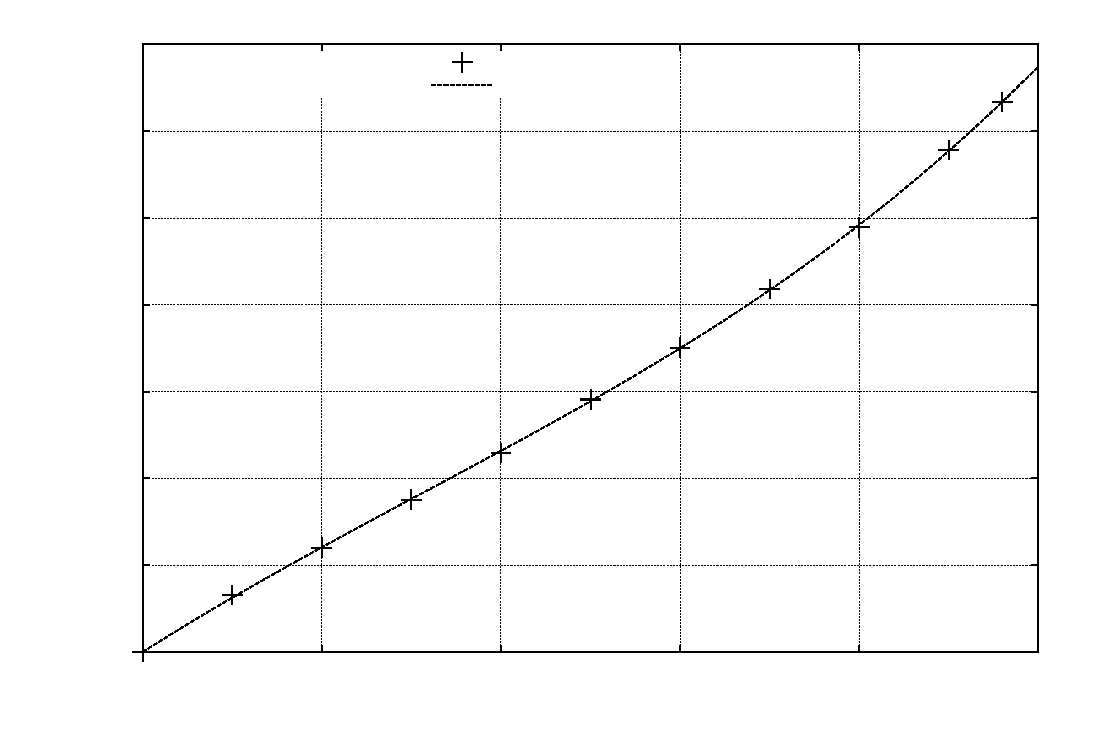
\includegraphics{DTP}}%
    \gplfronttext
  \end{picture}%
\endgroup

\caption{Ionizační ztráty v závislosti na tlaku}
\label{g:deltaT}
\end{graph}

\begin{graph}[htbp] 
\centering
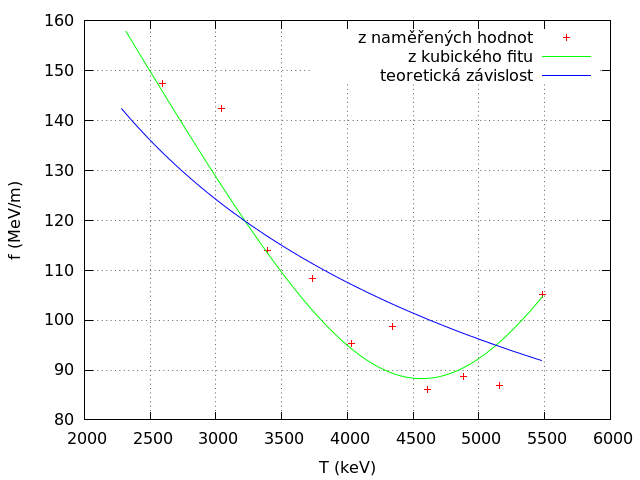
\includegraphics[width=\textwidth-2cm]{datos/f.png}
\caption{Specifické ionizační ztráty}
\label{g:f}
\end{graph}


Měřili jsme spektrum vzorku \Pudev~s příměsí \Puosm, výsledky jsou v tabulce \ref{t:vysledkyPu}. Podle \eqref{Pu} jsme spočítali jejich poměr
\begin{equation*}
\frac{N(^{238}\text{Pu})}{N(^{239}\text{Pu})}= (\num{3.8(3)})\cdot\num{e-5} \,.
\end{equation*}
Z toho máme relativní zastoupení 
\begin{equation*}
\eta(^{238}\text{Pu}) = \SI{0.0038(3)}{\percent}
 \,, \qquad \qquad \eta(^{239}\text{Pu} = \SI{99.996(1)}{\percent}
\end{equation*}







\begin{tabulka}[htbp]
\centering
\begin{tabular}{c|ccc|cc}
izotop & $T$ (\si{\keV}) & FWHM (\si{\keV}) & výtěžek (cps) & $T_{1/2}$ (\si{yr}) & $T_{\text{tab}}$ (\si{\keV}) \\\hline
\Pudev  &\num{5136.0(4)} & \num{110.07} & \num{16910(130)} & \num{24130} & \num{5142.90} \\ 
\Puosm  &\num{5475(3)} & \num{109.15} &   \num{178(14)}  & \num{87.71}  & \num{5499.21} \\ 

\hline
\end{tabular}
\caption{Naměřené píky při různých tlacích}
\label{t:vysledkyPu}
\end{tabulka}





%Diskuze výsledků
\section*{Diskuze}

%Závěr
\section*{Závěr}


\printbibliography[title={Seznam použité literatury}]

\end{document}